\chapter{Implementace}\label{ch:implementace}

Tato příloha popisuje technické provedení dílčích částí práce. Především dokumentuje obecné procesy shodující se pro všechny porovnávané \CICD systémy. Konkrétní detaily jednotlivých systémů jsou zdokumentovány v hlavní části práce.

Self-hosted \CICD systémy jsem nasazoval v lokálním virtuálním stroji za pomoci prostředí Vagrant~\cite{hashimoto-vagrant,susanka-vagrant}. Pro tuto práce jsem využil současně nejaktuálnější verzi \code{2.2.2}. Jako virtualizační jádro jsem použil Oracle VirtualBox~\cite{virtualbox} ve verzi \code{5.2.22-126460-OSX}.

Jako základ každé instalace jsem vybral Ubuntu~\cite{ubuntu}, která je podle W3Techs s 38,1 \% nejpoužívanější Linuxová distribuce~\cite{w3techs-stats}. Zvolil jsem aktuální vydání LTS (long-term support) \code{18.04}, oficiálně publikované jako Vagrant box \code{ubuntu/bionic64}.

K nainstalování závislostí na čistý operační systém i k instalaci samotných aplikací jsem využil software Chef~\cite{chef}. Jde o systém pro správu konfigurace a podporuje vývoj ve stylu \textit{Infrastructure as Code} (infrastruktura v kódu, oproti „klikacímu“ nastavování někde v \glstext{GUI}). Všechny konfigurace a nastavení systémů jsem tak mohl verzovat a sdílet na přiloženém médiu. Veškeré popsané experimenty by tak měly být naprosto opakovatelné a spustitelné s minimem další práce.

Pro každou komponentu jsem vytvořil samostatný virtuální stroj. Pro zjednodušení práce jsem ručně přidělil každému stroji IPv4 adresu z privátního bloku \code{10.0.0.0/24}. Nezprovozňoval jsem DNS server a pouze jsem každému stroji nastavil jména ostatních stanic v \code{/etc/hosts}. Aby spolu stanice mohli komunikovat, především aby \CD servery měli přístup k \HTTP serverům, přiděluje se každé stanici stejný předgenerovaný RSA klíč. To je špatná praxe, je to nebezpečné a pro praktické použití je to nepřípustné. V tomto případě jsem ale pro testování volil praktickou možnost, které zároveň nabízí 100\% opakovatelnost.

V ukázkových projektech jsem potřebovat využít samostatné git repozitáře, protože to velká část \CICD systémů vyžaduje, ale chtěl jsem zároveň verzovat celou diplomovou práci v jednom repozitáři. Vědomně jsem nepoužil git submodules, protože chci co nejjednodušší systém a distribuovat celou práci mimo přiloženého media i online, s případnými aktualizacemi. Místo toho jsem vytvořil v každém ukázkovém projektu git repozitář, který se používá pouze při pushování do \CICD systému. Potom složku \code{.git} přesunu předpřipraveným scriptem \code{make unstage}, případně vrátim příkazem \code{make stage}. Toto řešení mi dále umožňuje rychle iterovat nad projekty, nahrávat změny do \CICD a upravovat, a po dolazení pak verzovat výsledky bez nutnosti commity rebasovat a přejmenovávat.

\afterpage{
    \begin{iffigure}
        \centering
        \makebox[\textwidth][c]{
            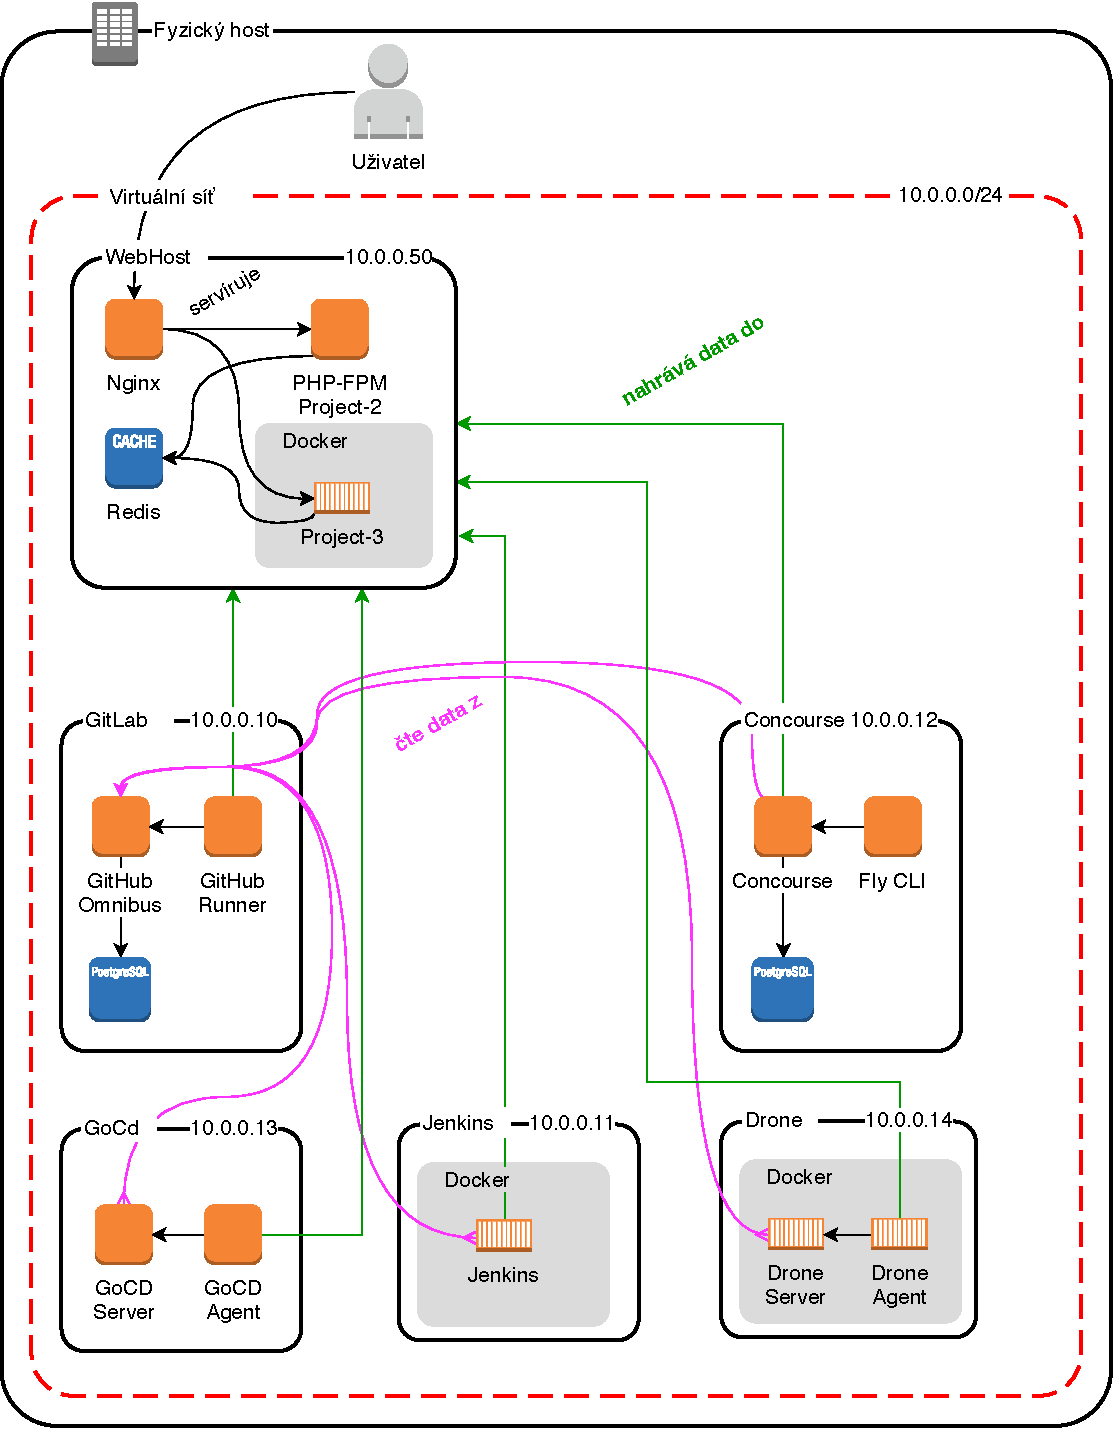
\includegraphics[width=1.2\textwidth]{media/test-architecture.pdf}
        }
        \caption{Diagram znázorňující propojení virtuálních strojů a dalších komponent na lokální síti.}
        \label{fig:test-architecture}
    \end{iffigure}
}

\section{GitLab}
    K instalaci GitLabu jsem použil oficiální návod pro systém Ubuntu. Vytvořil jsem vlastní -- velmi jednoduchý -- předpis pro systém Chef. Záměrně jsem nepoužil žádný z řady existujících Chef cookbooks, abych měl přehled co instalace obnáší. Dále můj cookbook konfiguruje GitLab přímo pro potřeby této práce.

    Po instalaci je automaticky zaregistrován uživatel \code{root} s přednastaveným heslem \code{CVUT\_FIT}. Repozitáře jsem nenascriptoval a je potřeba je ručně vytvořit. Dále je potřeba uživateli nastavit veřejný SSH klíč, který slouží ke sprárování identity při práci s repozitáři.

\section{Jednoduchý webserver}
    Pro nasazení ukázkových projektů jsem vytvořil nový čistý virtuální stroj. Abych mohl provozovat na \HTTP portu více aplikací rozlišených podle host, nainstaloval jsem na server nginx. Pro statický projekt jsem pouze nakonfiguroval cestu k veřejnému adresáři. Deploy probíhá dvoufázově: nejprve se na server nahrají statické zdroje (javascripty, kaskádové styly, \ldots) a poté se přepíší \glstext{HTML} soubory které na ně odkazují. Dynamické review apps jsem na straně web serveru implementoval proměnným názvem serveru:

        \begin{minted}[frame=lines,framesep=2mm,linenos]{ruby}
server_name "~^(?<domain>[\w-]+)\.p1\.ditemiku\.local$";
root /srv/p1-$domain;
        \end{minted}

    Pro druhý ukázkový projekt jsem nainstaloval PHP-FPM a nechal uživatelské požadavky přeposílat přes fastcgi. Deploy jsem implementoval podobně jako u statického webu. Díky tomu, že PHP používá opcache -- tzn. nečte a neparsuje při každém požadavku zdrojové soubory znovu -- stačí nahrát všechny soubory a pak opcache smazat. Toho se nejsnadněji docílí reloadem PHP-FPM masteru, který postupně vypne staré workery a zapne nové.

    Třetí projekt -- aplikaci v kontejneru -- jsem nasadil pomocí Docker Swarm, kde jsem z webserveru udělal jednouzlový server. Oproti čistému dockeru Swarm nabízí snažší správu závislostí pomocí \code{docker-compose.yml} a částečně umí udělat tzv. rolling update bez výpadku. V \CI systému se staví samotný docker image a nahraje se do sdíleného registru (Docker Registry) pod dvěma tagy: \code{latest} a \code{\$CI\_COMMIT\_SHA}. To je hash z verzovacího systému, který právě \CI systém staví. Díky otagování každé verze pak máme snažší správu: víme v jaké verzi aplikace zrovna běží a můžeme případně udělat rychlý rollback na starší verze. V případě že bychom pouze používali tag \code{latest}, tuto informaci bychom neměli a při rollbacku bychom museli spustit znova celou \CI pipeline.
